\chapter{A Unified Orbital Model of Delocalized and Localized Currents in Monocycles, from Annulenes to Azabora-Heterocycles}
\label{chap_huckel}
\footnotetext{Reproduced with permission: ``A Unified Orbital Model of Delocalized and Localized Currents in Monocycles, from Annulenes to Azabora-Heterocycle'', \mbox{A. Soncini}, \mbox{C. Domene}, \mbox{J. J. Engelberts}, \mbox{P. W. Fowler}, \mbox{A. Rassat}, \mbox{J. H. van Lenthe}, \mbox{R. W. A. Havenith} and \mbox{L. W. Jenneskens}, \textit{Chem. Eur. J.} \textbf{2005}, \textit{11}, 1257-1266\ \ \ \textbf{www.chemeurj.org}\ \ \ \copyright 2005 Wiley-VCH Verlag GmbH \& Co. KGaA, Weinheim}

\ifthenelse{\boolean{wholethesis}}{\relax}{\begin{center}\textit{Generated on \today\ at \currenttime}\end{center}}

\noindent\textbf{Abstract:} Why are some $4n+2$ $\pi$ systems aromatic, and some not?  The ipsocentric approach to calculation of the current density induced in a molecule by an external magnetic field predicts a four-electron diatropic (aromatic) ring current for $4n+2$ $\pi$, and a two-electron paratropic (anti-aromatic) current for $4n$ $\pi$ carbocycles. With the inclusion of an electronegativity parameter, an ipsocentric frontier-orbital model also predicts the transition from delocalized currents in carbocycles to nitrogen-localized currents in alternating azabora-heterocycles, which rationalizes the differences in (magnetic) aromaticity between these iso-electronic $\pi$ conjugated systems.  \textit{Ab initio} Valence Bond calculations confirm the localization predicted by the na\"ive model, and coupled Hartree-Fock calculations give current-density maps that exhibit the predicted delocalized-to-localized/carbocycle-heterocycle transition.
\clearpage

% jeroene - supporting information

\section{Introduction}
\lettrine{\initial{P}}{}lanar conjugated carbocyclic compounds show a strong link between $\pi$ electron count and molecular properties. H\"uckel's long-standing $4n+2$ rule distinguishes aromatic from anti-aromatic cycles, and correlates the energetics of these systems with their characteristic magnetic properties \cite{r01}. However, the periodic table offers wide possibilities for construction of iso-electronic heterocycles, and for many of them, direct transferability of the implied relationship between aromaticity and electron count is questionable or even counterfactual.  The replacement of CC by BN, for example, is known to lead to marked differences in magnetic properties \cite{r02}: the strong ring currents of the carbocycle vanish in the iso-electronic azabora-heterocycles, B$_{N/2}$N$_{N/2}$H$_N$ (\textbf{1}-\textbf{3}).  Herein we show that a simple frontier-orbital model of induced currents can in fact cope with both extremes, predicting the transition from delocalized to localized magnetic behavior that is found in full \textit{ab initio} current-density maps.
\begin{figure} [htp]
\begin{center}
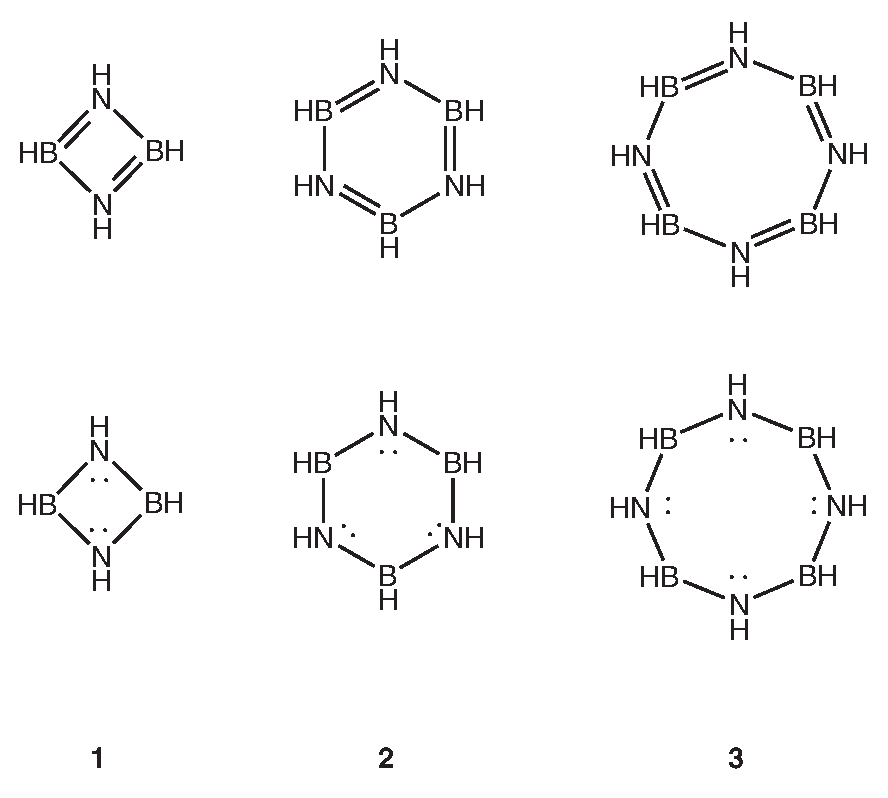
\includegraphics[width=3.4in]{huckel/figures/scheme1.eps}
\end{center}
\end{figure}

The ipsocentric model \cite{r03,r04,r05} gives an accurate account of $\pi$ ring currents in planar carbocycles in terms of frontier-orbital contributions. The hallmarks of aromaticity and anti-aromaticity on the magnetic criterion \cite{r06,r07,r08,r09}, that is, the \textit{diatropic} currents of $4n+2$ systems and \textit{paratropic} currents \cite{r10} of planar $4n$ systems, are attributed in this model to four and two frontier electrons, respectively \cite{r04}. In both cases, the sense of the ring current follows directly from the symmetry properties of the HOMO--LUMO transition, and the predictions of a simple orbital theory are borne out in full \textit{ab initio} calculation of current-density maps \cite{r03,r04}. For the $4n+2$ heterocycles, borazine and boroxine, however, \textit{ab initio} maps show only \textit{localized} circulation of the $\pi$ electrons around the electronegative nuclei \cite{r02}.  How does the simple orbital model deal with this dichotomy?  In particular, why does it not predict ring currents for \textit{all} planar $4n$ and $4n+2$ $\pi$ systems? It is shown here that a generalization of the pictorial orbital model is able to account for both the presence of global currents in the carbocycles, and their absence in boron-nitrogen analogues such as borazine (\textbf{2}) and the eight-membered borazocine (\textbf{3}).

\section{Results and Discussion}

\subsection{The Aromaticity Analogy}

The considerations of magnetic aromaticity have their counterparts in the chemistry of these boron-nitrogen systems.  Although 6$\pi$ electron borazine (\textbf{2}) was originally called ``an inorganic benzene''\footnote{For recent summaries of the history of the discussion on the putative aromatic character of borazine, see, for example \cite{r11} and \cite{r11b}} and believed to have a resonance
energy similar to that of benzene, it was soon recognized that it had few reactions typical of aromatic systems.  For instance, borazine gives a tris-adduct with hydrogen chloride \cite{r12}. It is now generally agreed that borazine is not aromatic. In contrast to benzene, the $\pi$ electrons are localized on the more negative nitrogen atoms, even if some chemical behavior is reminiscent of that of benzene (e.g. formation of a weakly puckered hexaethylborazine tricarbonyl chromium complex) \cite{r13}.

The parent compounds B$_{N/2}$N$_{N/2}$H$_N$ with $N \ne 6$ have not been synthesized, although many derivatives of the homologues diazadiboretidine (also known as diazadiboretane, diazadiborete) (\textbf{1}) and borazocine (tetrazaborocine, tetrazaborocane) (\textbf{3}), have been prepared \cite{r14}. Interconversions between them (and with borazine) are possible, and their chemical properties differ strongly from those of the corresponding 4 $\pi$ and 8 $\pi$ carbocycles.  For instance, the four-membered ring survives thermal elimination of isobutene from a \textit{tert}-butyl derivative \cite{r14}.  Thus, in spite of their $4n$ $\pi$ electrons, these systems do not show the reactivity expected for an anti-aromatic molecule.  This again can be attributed to a localization of the $\pi$ electrons onto the more electronegative nitrogen atoms.  Similarly, energy calculations \cite{r11b,r15} suggest that \textbf{1} is less anti-aromatic than cyclobutadiene, in agreement with the H\"uckel prediction that
the anti-aromaticity in X$_2$Y$_2$H$_4$-type four-membered rings decreases with increasing electronegativity difference between X and Y \cite{r16}.  By using the ipsocentric model, we show here that diazadiboretidine (\textbf{1}), borazine (\textbf{2}) and borazocine (\textbf{3}) are in all fact \textit{non-aromatic}.

\subsection{Aromaticity, Ring Currents and Frontier Orbitals}

If aromaticity is to be defined by magnetic criteria \cite{r09}, then what is needed for its theoretical characterization is a reliable account of the currents induced by an external magnetic field, since susceptibility, nuclear shielding and other response properties are all integrals of this current density.  Realistic current-density maps can now be obtained by a computationally efficient procedure, the ipsocentric method, which avoids the gauge dependence problem by taking each point in space as an origin of the vector potential generating the magnetic field \cite{r17,r18}. This choice has the important conceptual advantage of yielding a unique decomposition into non-redundant orbital contributions \cite{r03}. The total current density is obtained as a sum over transitions from occupied to unoccupied orbitals, governed by symmetry rules, and modulated by energy denominators.

For a planar molecule in a perpendicular magnetic field, the symmetries determining the sense of circulation of the induced current about the molecular origin are those of in-plane translations ($T_x$, $T_y$) and the in-plane rotation, ($R_z$). A simple but powerful symmetry rule can be deduced. If the symmetry of a product of occupied and unoccupied orbitals contains that of $T_x$ or $T_y$, but not that of $R_z$, the contribution of the transition to the current has the \textit{diatropic} sense, and if it contains the symmetry of $R_z$, but not $T_x$ or $T_y$, the contribution has the reverse \textit{paratropic}, sense. If neither symmetry is present, the transition is inactive; if both, more detailed analysis is needed \cite{r03,r19}. On the magnetic criterion, the resultant of all such contributions determines aromaticity or anti-aromaticity (net diatropicity or paratropicity of ring current) of a monocycle. As the contributions are weighted by orbital energy \textit{differences}, frontier orbitals generally dominate.

\subsection{Currents in Carbocycles}

Current-density maps from \textit{ab initio} calculations \cite{r04} on the archetypal carbocycles, benzene and (planarized \cite{r20a,r20b}) cyclooctatetraene (COT) are shown in Figure \ref{ch5.fig.f01}. For each
molecule, the maps show total $\pi$ and $\sigma$ contributions to induced current density.  As expected, the currents arising from the $\pi$ electrons are respectively strongly diatropic in benzene and strongly paratropic in COT. Currents are dominated by HOMO contributions in both cases.
\begin{figure}
\begin{center}
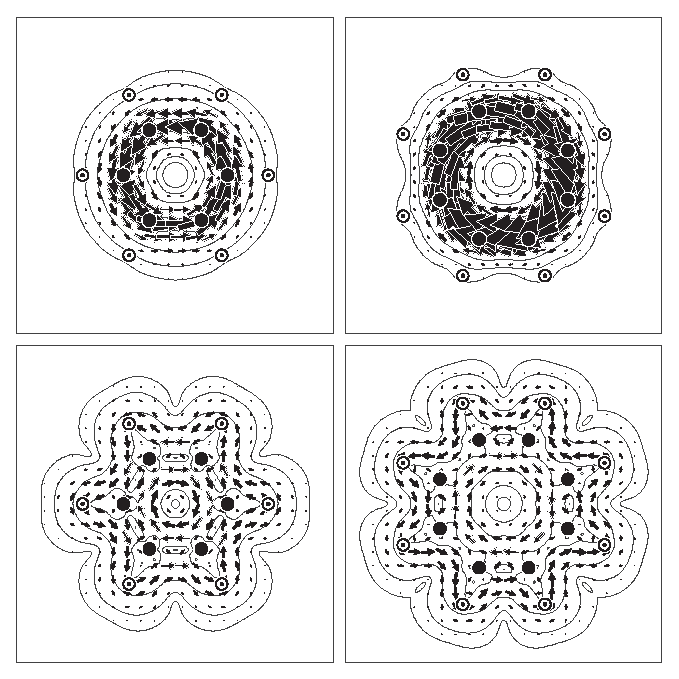
\includegraphics[scale=1.3]{huckel/figures/fig1.eps}
\caption{Maps of the current density induced by a perpendicular external magnetic field in benzene (left) and
(planar) cyclooctatetraene (right).  Contributions of the $\pi$ (top) and $\sigma$ orbitals (bottom), calculated in the
RHF/6-31G$^{**}$ ipsocentric approach, plotted at one bohr above the molecular plane.  Anti-clockwise circulations
are diatropic, clockwise circulations paratropic. Carbon ($\bullet$) and hydrogen ($\odot$).}
\label{ch5.fig.f01}
\end{center}
\end{figure}

An angular momentum analysis shows how the symmetry rules account for these features. The H\"uckel $\pi$ molecular
orbitals of a cycle of $N$ identical atoms in full $D_{N\mathbf{h}}$ symmetry have well defined angular momentum properties
with respect to the principal axis. At each successive energy level, the quantum number, $\lambda (=0,1...,N/2)$,
increases by one. In a cycle with $N = 4n+2$ electrons, the HOMO and LUMO correspond to $\lambda = n$ and
$\lambda = n+1$, whereas for a cycle with $N = 4n$ electrons, in the closed-shell configuration obtained on
distortion to $D_{(N/2)\mathbf{h}}$ symmetry, the HOMO and LUMO derive from splitting of a pair of originally degenerate
orbitals with $\lambda = n$.

The canonical molecular orbitals are the \textit{delocalized} set ${\Psi_{\lambda,c/s}}$, producing uniform $\pi$ charge distribution on all C atoms. Functions {$\Psi_{\lambda,c}$} and {$\Psi_{\lambda,s}$} (degeneracy $d_\lambda$) have coefficients on center $r$ equal to $\sqrt{d_{\lambda/N}}\cos(2 \pi \lambda r/N)$ and $\sqrt{d_{\lambda/N}}\sin(2 \pi \lambda r/N)$, respectively \cite{r21}. Unless $\lambda = 0$ (or $N/2$, if allowed) the two functions share a single, well-defined angular momentum and are degenerate. For $\lambda = 0$ and $\lambda = N/2$, the sine partner vanishes identically. For other $\lambda$, the sine/cosine form is simply a choice that gives
convenient nodal properties.

When orbitals have well defined values of $\lambda$, the symmetry selection rules
for occupied-to-unoccupied transitions reduce to the following \cite{r04}: a diatropic contribution arises from a transition in which $\Delta\lambda = +1$, a paratropic contribution arises from a transition in which $\Delta\lambda = 0$. Thus, for a $4n+2$ cycle in maximum symmetry, only the HOMO--LUMO transition is active, and is responsible for the entire (4-electron) diatropic current. For a $4n$ cycle in the lower symmetry of the closed shell, two types of transition are active: the HOMO--LUMO transition leads to a 2-electron paratropic contribution, and HOMO-1--LUMO, HOMO--LUMO+1 to diatropic contributions.  Here, the smaller HOMO--LUMO splitting ensures dominance of the paratropic current. Decomposition of the carbocycle \textit{ab initio} $\pi$ maps into orbital contributions confirms the above analysis in detail \cite{r04}.

\subsection{A Model for Currents in Azabora-Heterocycles}

To adapt the pictorial molecular orbital analysis to the ipsocentric model for currents in the alternating heterocycles
such as borazine (\textbf{2}) and homologues \textbf{1} and \textbf{3}, it is sufficient to include one extra feature.
The method for dealing with heteroatoms in H\"uckel theory is to modify Coulomb and/or resonance integral parameters:
for B and N (as zero and two-electron donors), recommended parameters are $\alpha_B = \alpha -\beta$ and
$\alpha_N = \alpha + 1.5\beta$ \cite{r22a,r22b}. H\"uckel calculations using $\alpha_B = \alpha -1.1\beta$ and
$\alpha_N = \alpha + 1.5\beta$ have been reported for \textbf{1} to \textbf{3} \cite{r16}. The simplest model of an
equilateral B$_{N/2}$N$_{N/2}$H$_N$ cycle that allows for the differing electronegativities of B and N makes symmetrical
changes to the Coulomb parameters, that is, $\alpha_B = \alpha -\eta\beta$ and $\alpha_N = \alpha +\eta\beta$, where 
$\eta$ is positive.  Variation of the dimensionless quantity $\eta$ from $0$ to $\approx 1$ thus gives a one-parameter
model for correlating properties of annulenes and BN cycles.

The implications are now worked out in detail for six- and eight-cycles, as representatives of $4n+2$ and $4n$ $\pi$
systems, respectively.  Direct solution of the H\"uckel problem with modified $\alpha$ values gives energy levels {$\epsilon$}
and molecular orbitals {$\phi$}, from which consequences for ring currents can be deduced. In the limit $\eta = 0$,
the canonical molecular orbitals are {$\Psi_{\lambda,c/s}$}; when $\eta \ne 0$, they are linear combinations
of this starting set.

\subsubsection{Currents in the Six-Membered Cycle}

The secular equations for the alternating six-membered cycle
have maximal symmetry $D_{3\mathbf{h}}$ ($\eta \ne 0$) or $D_{6\mathbf{h}}$ ($\eta = 0$). The energies are ($D_{3\mathbf{h}}$ /$D_{6\mathbf{h}}$ labels,
$d_\lambda$ = degeneracy): 

\begin{math}
\\
\epsilon_0 = \alpha + \sqrt{4+\eta^2}\beta(\mathrm{A}_2''/\mathrm{A}_{2\mathrm{u}}), d_\lambda = 1;
\\
\\
\epsilon_1 = \alpha + \sqrt{1+\eta^2}\beta(\mathrm{E}''/\mathrm{E}_{1\mathrm{g}}), d_\lambda = 2;
\\
\\
\epsilon_2 = \alpha - \sqrt{1+\eta^2}\beta(\mathrm{E}''/\mathrm{E}_{2\mathrm{u}}), d_\lambda = 2;
\\
\\
\epsilon_3 = \alpha - \sqrt{4+\eta^2}\beta(\mathrm{A}_2''/\mathrm{B}_{2\mathrm{g}}), d_\lambda = 1.
\\
\\
\end{math}

When $\eta$ is non-zero, functions with different $\lambda$ are allowed to mix according to their symmetries in
the lower $D_{3\mathbf{h}}$ group, that is, in $\mathrm{A}_2''$, $\lambda = 0$ mixes with $\lambda = 3$, and in
$\mathrm{E}''$, $\lambda = 1$ mixes with $\lambda = 2$ (retaining the sine/cosine distinction).  As $\eta$
increases, the degree of mixing increases, and is described by angles $\mu$ and $\nu$, where
$\eta=2\tan2\mu=\tan2\nu$:

\begin{math}
\\
\phi_{0,c} = \cos \mu \psi_{0,c} - \sin \mu \psi_{3,c},
\\
\\
\phi_{1,c} = \cos \nu \psi_{1,c} - \sin \nu \psi_{2,c}, \phi_{1,s} = \cos \nu \psi_{1,s}+\sin \nu \psi_{2,s},
\\
\\
\phi_{2,c} = \sin \nu \psi_{1,c} + \cos \nu \psi_{2,c}, \phi_{2,s} = -\sin \nu \psi_{1,s}+\cos \nu \psi_{2,s},
\\
\\
\phi_{3,c} = \sin \mu \psi_{0,c} + \cos \mu \psi_{3,c}.
\\
\\
\end{math}

At $\eta= 0$, $\mu$ and $\nu$ are zero; in the limit of large $\eta$, the molecular orbitals of the alternating 6-cycle
become exact 50:50 mixtures, with $|\mu| = |\nu| = 45$\degrees. When $\eta=1$, $\phi_{1,c/s}$ still contains 95\% of the
benzene $\psi_{0,c}$  ($|\mu | = 13.3$\degrees), but the HOMO pair, $\phi_{1,c/s}$, contains a 15\% admixture of the
benzene LUMO,  $\psi_{2,c/s}$  ($|\nu| = 22.5$\degrees).  Figure \ref{ch5.fig.f02}(a) shows the correlation of orbitals and
energies with $\eta$ for the 6-cycle. H\"uckel $\pi$ charges reflect this shift with respect to the uniform charge distribution
of benzene, with \mbox{$1 \pm \frac{1}{2} (\frac{1}{\sqrt{5}} + \sqrt{2}) \approx 1.62$} and 0.38 $\pi$ electrons on the nitrogen and
boron atoms when $\eta=1$.  As $\eta$ increases, bonding orbitals concentrate onto electronegative nitrogen atoms, and
anti-bonding orbitals on the electropositive boron atoms, the functions becoming more ``localized''. 
\begin{figure}[htp]
\begin{center}
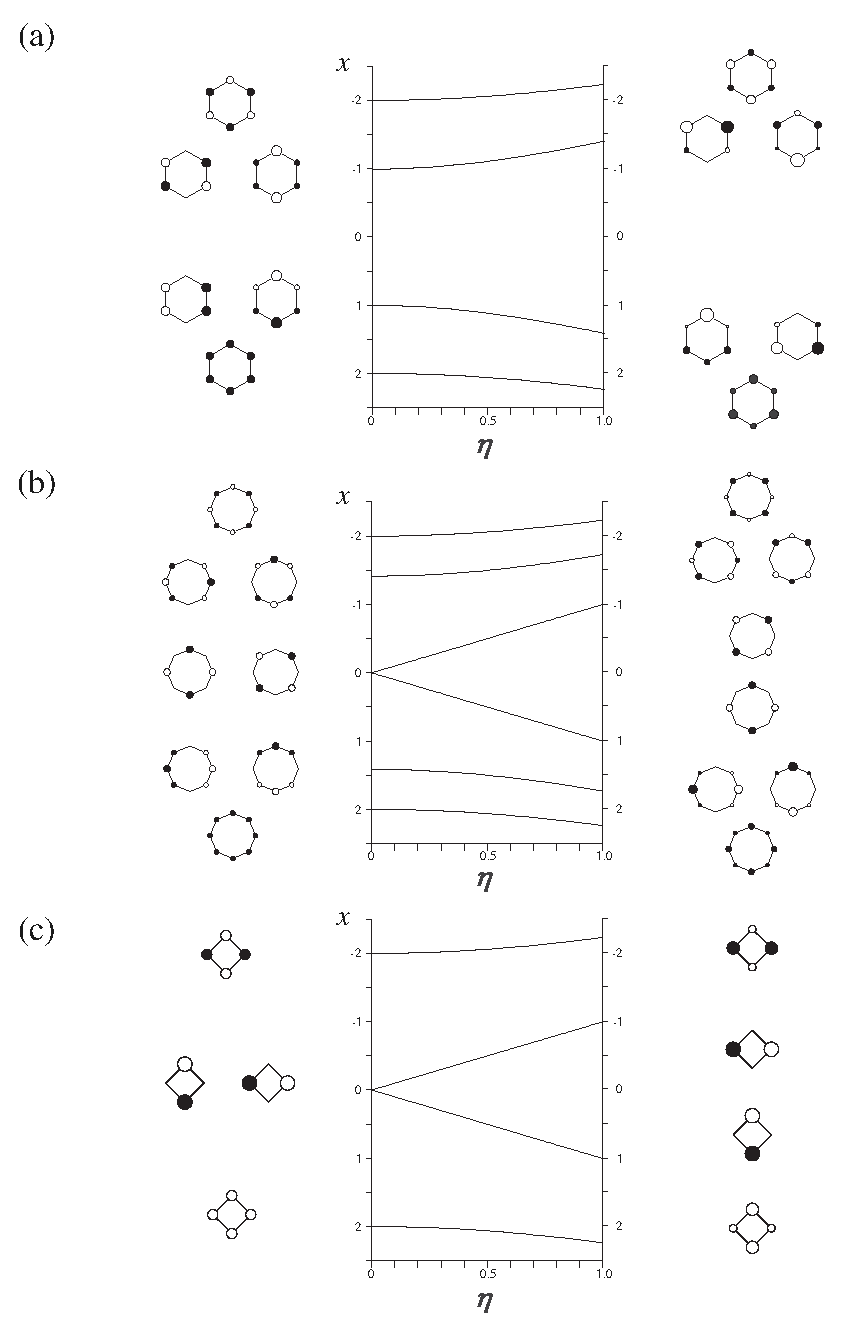
\includegraphics[scale=0.95]{huckel/figures/fig2.eps}
\end{center}
\caption{Correlation diagrams of energy and orbital composition in a H\"uckel model of \mbox{a) B$_3$N$_3$H$_6$,} 
\mbox{b) B$_4$N$_4$H$_8$} and \mbox{c) B$_2$N$_2$H$_4$,} as modeled by the single parameter $\eta$, where
$\alpha_\mathrm{B}=\alpha-\eta\beta$ and $\alpha_\mathrm{N}=\alpha+\eta\beta$. The graphs show the
variation of orbital energy, $x=(\epsilon-\alpha)/\beta$, with $\eta$.}
\label{ch5.fig.f02}
\end{figure}

The mixing has crucial consequences for predicted currents. At $\eta=0$, the dominant HOMO--LUMO transition responsible
for the ring current of the carbocycle is from {$\psi_{1,c},\psi_{1,s}$} to {$\psi_{2,c},\psi_{2,s}$}, for which $\Delta\lambda=1$; the
transition is therefore purely translational and contributes \textit{only} diatropic current.  For all $\eta>0$, as HOMO and LUMO
each contain $\lambda = 1$ and $2$ contributions, the transition includes $\Delta\lambda = 1$ and $0$ components, and the current
gains partial paratropic character.  The global diatropic current of benzene therefore weakens as $\eta$ increases.

A first interpretation of the effect of progressive orbital mixing on the ring current in a $4n+2$ cycle can be found by using
the simplest approach, the H\"uckel-London model \cite{r06}.  In this model, as formulated by McWeeny \cite{r23}, the ring current
per unit area of a cycle is proportional to the reduced bond current, $J_{rs}$, where $p_{rs}$ is the $\pi$ bond-order between
adjacent atoms $r$ and $s$ and $\overline{\pi}_{rs,rs}$ is the imaginary bond-bond polarizability \cite{r01}. 

\begin{math}
\\
J_{rs}=(p_{rs}+\beta\overline{\pi}_{rs,rs})\beta
\\
\end{math}

In a monocycle, $J$, $p$ and $\overline{\pi}$ are independent of the choice of adjacent pair. For benzene, $p=\frac{2}{3}$ and
$\overline{\pi}=-\frac{5}{9}\beta^{-1}$. For borazine with $\eta=1$, a straightforward calculation gives $p=\frac{1}{3}(\frac{2}{\sqrt{5}}+
\frac{1}{\sqrt{2}})$ and $\overline{\pi}=-\frac{1}{9}(\sqrt{5}+\frac{13}{4\sqrt{2}})\beta^{-1}$, from which the borazine:benzene
ratio of ring current intensity, assuming an equal ring area, is $(\frac{1}{\sqrt{5}}-\frac{1}{4\sqrt{2}})\approx 0.27$. This ratio
tends to zero as the electronegativity difference parameter $\eta$ tends to infinity. Thus, this crude model, in which current
is constrained to flow along the straight lines between adjacent atoms, predicts that an increase in $\eta$ leads to diminution
and eventual extinction of the global diatropic current. 

The picture can be refined by allowing for the spatial extent of the current outside the direct line of centers. The pseudo-$\pi$
model \cite{r24} includes explicit basis functions, and simulates $\pi$ ring currents by using a $\sigma$ model based on
the exact symmetry equivalence between the $\sigma$ orbitals of cyclic H$_N$ atoms and the $\pi$ orbitals of the
$N$-membered carbocycle. It turns out that ipsocentric \textit{in-plane} currents calculated for the H$_N$ system with
a minimal basis set give an excellent match to the \textit{out-of-plane} currents of the carbocycle calculated with a large
basis set. Figure \ref{ch5.fig.f03} presents a pseudo-$\pi$ simulation of the heterocyclic ring in which the boron and nitrogen
atoms are modeled by one-electron atoms with nuclear charges of $+0.7e$ and $+1.3e$, each carrying STO-3G $s$ and $p$
functions (exponent $1a_{0}^{2}$), the charge difference playing the role of the $\eta$ parameter in the H\"uckel analysis,
and the in-plane $p$ functions giving radial flexibility to charge and current densities. 
\begin{figure}[htp]
\begin{center}
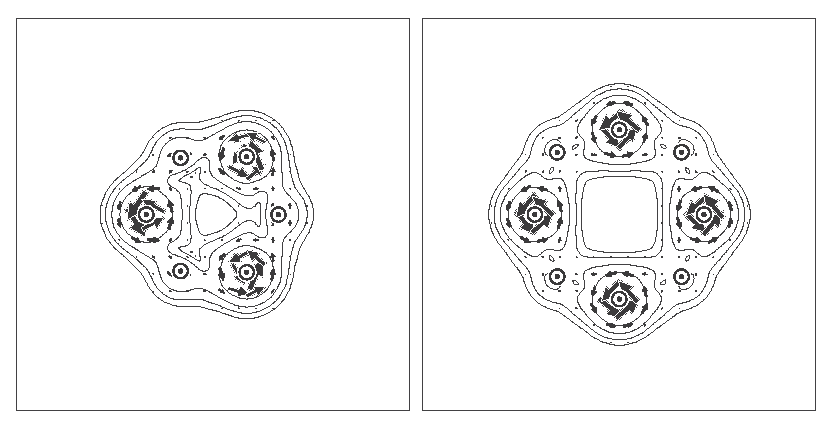
\includegraphics{huckel/figures/fig3.eps}
\end{center}
\caption{\textit{Pseudo}-$\pi$ simulations of induced current density in B$_{N/2}$N$_{N/2}$H$_N$, with $N=6$ (left) and 
$N=8$ (right). In these molecules intense in-plane local circulations around the nitrogen centers in this pseudo-$\pi$ model
indicate out-of-plane $\pi$ circulations of similar strength. Here the symbol $\odot$ denotes the pseudo-hydrogen centers
representing the boron and nitrogen atoms in the model. Anti-clockwise circulations are diatropic, clockwise circulations
paratropic.}
\label{ch5.fig.f03}
\end{figure}
Pure symmetric arguments predicted
opposed paramagnetic and diamagnetic currents; the pseudo-$\pi$ map shows that they occupy different regions of space,
with diamagnetic circulation on the inside of the ring, the net effect being a set of circulations centered on electronegative atoms.
In the graph-theoretical H\"uckel-London model, this spatial pattern of opposed local currents was expressed as a reduction
of the sole available parameter, the bond current. Both models therefore essentially agree on the effect of the electronegativity
difference on the ring current.

\subsubsection{Currents in the Eight-Membered Cycle}

For the alternating eight-membered cycle, the maximal symmetry is $D_\mathrm{4h}$ ($\eta \ne 0$) or $D_\mathrm{8h}$
($\eta = 0$) and the energy levels $\varepsilon_{\lambda}$($D_\mathrm{4h}/D_\mathrm{8h}$ labels, $d_\lambda=$
degeneracy) are:

\begin{math}
\\
\varepsilon_0=\alpha+\sqrt{4+\eta^{2}}\beta \mathrm{(A_{2u}/A_{2u})}, d_\lambda=1;
\\
\\
\varepsilon_1=\alpha+\sqrt{2+\eta^{2}}\beta \mathrm{(E_{g}/E_{1g})}, d_\lambda=2;
\\
\\
\varepsilon_{2}^{\pm}=\alpha \pm \eta\beta \mathrm{(B_{1u}+B_{2u}/E_{2u})}, d_\lambda=2 \mathrm{\ at\ } \eta=0;
d_\lambda=1+1 \mathrm{\ at\ } \eta \ne 0;
\\
\\
\varepsilon_3=\alpha-\sqrt{2+\eta^{2}}\beta \mathrm{(E_{g}/E_{3g})}, d_\lambda=2;
\\
\\
\varepsilon_4=\alpha-\sqrt{4+\eta^{2}}\beta \mathrm{(A_{2u}/B_{2u})}, d_\lambda=1;
\\
\end{math}

In the carbocyclic system with full symmetry, the degeneracy of $\psi_{2,c}$ and $\psi_{2,s}$ leads to an open-shell configuration
which can be stabilized in various ways: distortion to $D_\mathrm{2d}$ leads to the tub-shaped equilibrium geometry of the free COT
molecule; in-plane relaxation to $D_\mathrm{4h}$ yields a geometry similar to those found in ``clamped''-substituted COT
systems \cite{r20a,r20b}. In spite of its bond alternation, planar $D_\mathrm{4h}$ COT retains fully delocalized orbitals and the ring
current of the equilateral carbocycle, as Figure \ref{ch5.fig.f01} shows \cite{r04,r20b}.

In the heterocyclic system, when $\eta \ne 0$, with the nitrogen atom as atom $0$, $\psi_{2,c}$ as the bonding and $\psi_{2,s}$
the anti-bonding partner, the assignment of labels B$_\mathrm{1u}$ and B$_\mathrm{2u}$ depends on the setting of $D_\mathrm{4h}$
within $D_\mathrm{8h}$. For a general value of $\eta$, the mixing of angular momentum components is again described by two
angles, $\mu$ and $\kappa$, with $\eta=2\tan 2 \mu = \sqrt{2} \tan 2 \kappa$.

\begin{math}
\\
\phi_{0,c} = \cos \mu \psi_{0,c} - \sin \mu \psi_{4,c},
\\
\\
\phi_{1,c} = \cos \kappa \psi_{1,c} - \sin \kappa \psi_{3,c}, \psi_{1,s} = \cos \kappa \psi_{1,s} + \sin \kappa \psi_{3,s},
\\
\\
\phi_{2,c} = \psi_{2,c}, \phi_{2,s} = \psi_{2,s},
\\
\\
\phi_{3,c} = \sin \kappa \psi_{1,c} + \cos \kappa \psi_{3,c}, \phi_{3,s} = - \sin \kappa \psi_{1,s} + \cos \kappa \psi_{3,s},
\\
\\
\phi_{4,c} = \sin \mu \psi_{0,c} + \cos \mu \psi_{4,c}.
\\
\end{math}

Note that functions $\psi_{2,c}$ and $\psi_{2,s}$, as the HOMO and LUMO, remain unmixed for all values of $\eta$, separated by a
gap that is linear in $\eta$, that is, $2\eta$. Each is perfectly localized, the HOMO on the nitrogen atom and the LUMO on the boron
atom. In contrast, with increasing values of $\eta$, the functions $\phi_{0,c}$, $\phi_{1,c}$, $\phi_{1,s}$, $\phi_{3,c}$, $\phi_{3,s}$ and
$\phi_{4,c}$ become increasingly localized on the electronegative atoms: when $\eta  = 1$, the nitrogen and boron atoms have
H\"uckel $\pi$ populations of \mbox{$1 \pm \frac{1}{2}(\frac{1}{2}+\frac{1}{\sqrt{3}}+\frac{1}{2\sqrt{5}}) \approx 1.65$} and $0.35$
electrons, respectively. When $\eta=1$, here representing planar B$_4$N$_4$H$_8$, $|\mu|=13.3$\degrees \ and
$|\kappa |=17.6$\degrees \ so that $\phi_{0,c}$ contains 5 \% of $\psi_{4,c/s}$ and HOMO--1 $\phi_{1,c/s}$ contains 10 \% of
$\psi_{3,c/s}$. Figure \ref{ch5.fig.f02}(b) shows the correlation of orbitals and energies with $\eta$ for the eight-membered cycle.
 
The symmetry argument for deducing the currents in $4n$ systems involves several steps. Initially ($\eta \approx 0$), the current is 
dominated by the HOMO--LUMO transition across a small energy gap. This $\Delta \lambda = 0$ transition generates an intense, purely
paratropic, ring current. As $\eta$ increases, the HOMO--LUMO gap opens, and the intensity of the current falls but remains paramagnetic.
Simultaneously, the separation of the \mbox{HOMO-1} and the LUMO and that of the HOMO and the LUMO+1, increase, but only slowly; both correspond
$\Delta \lambda = \pm 0$ diatropic contributions to current. Thus, as $\eta$ increases, the original global paratropic (anti-aromatic)
ring current is subject to intrinsic reduction and increasingly significant cancellation.

In the McWeeny form of the H\"uckel-London theory \cite{r23}, the ring current of the eight-membered cycle when $\eta$ is small is
dominated by the HOMO--LUMO contribution to the imaginary bond-bond polarizability, which is $-\frac{1}{16} \beta \eta$, and hence falls
sharply as $\eta$ increases from the planar-constrained form of COT (where $\eta=0$) to the heterocycle. When $\eta=1$, the
eight-membered cycle has $p=\frac{1}{2}(\frac{1}{\sqrt{3}}+\frac{1}{\sqrt{5}})$ and
$\overline{\pi}=-\frac{1}{8}(\frac{11}{3\sqrt{3}}+\frac{7}{2\sqrt{5}}+\frac{1}{2})\beta^{-1}$ to give bond currents
$J=\frac{\sqrt{3}}{72}+\frac{\sqrt{5}}{80}-\frac{1}{16}\approx -0.105$, which constitute a reduced but still net paratropic circulation.
If the ratio of the areas of the six- and eight-membered cycles is 9:16, a ring current of about a sixth of the strength of the
(diatropic) benzene current is implied. When, as for the six-membered cycles, the spatial extent of the current in the eight-membered
cycle is taken into account in a pseudo-$\pi$ calculation (Figure \ref{ch5.fig.f03}), the H\"uckel-London result is seen as a simplified
representation of the nitrogen-centered currents.

\subsubsection{Currents in the Four-Membered Cycle}

For the four-membered ring, B$_2$N$_2$H$_4$, the extinction of current with increasing $\eta$ follows the same pattern as that for the
eight-membered cycle. The four orbital energies are now $\epsilon_{0} = \alpha + \sqrt{4+\eta^{2}}\beta$,
$\epsilon_{1}^{\pm} = \alpha \pm \eta \beta$, again giving a linear HOMO--LUMO gap of $2\eta$ (see Figure \ref{ch5.fig.f02}c), and yielding
a paratropic current that weakens with $\eta$ and is increasingly cancelled by the diatropic current that arises from the transitions
across the HOMO--LUMO+1 and \mbox{HOMO-1}--LUMO gaps of $\eta+\sqrt{4+\eta^{2}}\beta$. In the H\"uckel-London theory, when $\eta=1$ the reduced
bond current for the four-membered ring remains net paratropic ($J=\frac{1}{4\sqrt{5}}; -0.138$) and corresponds to half the current
of a benzene ring which has $\frac{9}{4}$ times the area, and again represents the pattern of nitrogen-centered circulations in a more
detailed description.

\subsubsection{Generalization for $4n$ and $4n+2$ $\pi$ BN Heterocycles}

The results for the four-, six- and eight-membered cycles are generalizations for the $4n$ and $4n+2$ $\pi$ BN heterocycles, with
separate mechanisms, but equivalent results for the ring current in both cases. Consider an $[N]$-carbocycle, where $N$ is even.
As $\eta$ increases from 0, each bonding ($b$)/anti-bonding($a$) molecular orbital pair of the parent bipartite carbocycle, with angular
momenta $\Lambda_{b}$ and $\Lambda_{a}=N/2 - \Lambda_{b}$, which correspond to equal but opposite eigenvalues, mix to form a 
bonding/anti-bonding pair in the $[N]$-center BN heterocycle with energies $x_b = \sqrt{4\cos^{2}\tau_{\Lambda_b}+\eta^2}$ and
$x_a = -\sqrt{4\cos^2 \tau_{\Lambda_{a}}+\eta^2}$, where $\tau_\Lambda=2\pi\Lambda/N$, so that $x_b=-x_a$. The rotation describing the
mixing is parametrized by the angle $\omega_\Lambda=\frac{1}{2}\tan^{-1}(\eta/2\cos\tau_\Lambda)$, where $0 \le \omega_\Lambda \le \pi/4$.

When $N=4n+2$, $\Lambda_\mathrm{HOMO}=n$ and $\Lambda_\mathrm{LUMO}=n+1$, and the mixing angle $\omega_\Lambda$ is maximal for a given
value of $\eta$. As we have seen, this leads to a sufficiently large value of $\eta$ to disrupt the global ring current and eventual
localization. When $N=4n$, $\Lambda_\mathrm{HOMO}=\Lambda_\mathrm{LUMO}=n$, the original HOMO and LUMO carbocycle eigenfunctions remain
unmixed. Disruption of the global paratropic ring current is caused by the widening of the HOMO--LUMO gap, triggering cancellation of
the rotational HOMO--LUMO and translational \mbox{HOMO-1}--LUMO contributions.

\subsection{\textit{Ab Initio} Current-Density Maps in Azabora-Heterocycles}

To obtain \textit{ab initio} data on the currents in BN analogues of the $4n$ and $4n+2$ carbocycles, calculations were performed on B$_2$N$_2$H$_4$,
B$_3$N$_3$H$_6$ and B$_4$N$_4$H$_8$. The geometry of each molecule was optimized at the restricted Hartree-Fock (RHF) level with the 
6-31G** basis set and currents were calculated by using the ipsocentric approach at the coupled Hartree-Fock (CHF) level with the same
basis set. At this level of theory, B$_3$N$_3$H$_6$ and B$_4$N$_4$H$_8$ have planar structures with $D_\mathrm{3h}$ and $D_\mathrm{4h}$ symmetries,
respectively, whereas the planar structure of B$_2$N$_2$H$_4$ with $D_\mathrm{2h}$ symmetry is a transition state (imaginary frequency 116$i$
cm$^{-1}$) that leads to a shallow $C_\mathbf{2v}$ butterfly optimum, hinged at the BB diagonal, with a dihedral angle of 167\degrees.
Current-density maps were computed for both the constrained planar and the fully optimized structures of B$_2$N$_2$H$_4$. An alternative
geometry for B$_4$N$_4$H$_8$ is based on the occupation of the corners of a cube \cite{r25a}; this compact structure is slightly preferred
to the planar form, as determined with small basis sets \cite{r25b}, but lies 302 \mbox{kJ mol$^{-1}$} above it when calculated at the 6-31G**
level. All three planar molecules have uniform BN distances ($R$=1.4432, 1.4258, 1.4254 \AA, respectively).

These geometries are in general agreement with available experimental and theoretical data. The non-planarity of B$_2$N$_2$H$_4$ has been
noted in previous \textit{ab initio} calculations \cite{r26}, which gave a BN distance of 1.457 \AA, and although the parent molecule itself has not
been synthesized, X-ray structures of five substituted molecules \cite{r14} are known with mean BN distances varying between 1.430 and
1.486 \AA, and all are planar apart from the severely hindered tetra-\textit{tert}-butyl derivative. Borazine has been the subject of many
\textit{ab initio} calculations \cite{r27a,r27b,r27c,r27d,r27e,r27f}. The RHF/6-31G**-calculated BN distance of 1.4258 \AA\ in borazine compares with
1.4355$\pm$0.0021 \AA\ (gas electron diffraction \cite{r28a,r28b} and 1.429 \AA\ (X-ray \cite{r28c}). No experimental data are available for
parent B$_4$N$_4$H$_8$, but experimental and theoretical structural data on its derivatives have been reviewed by Gilbert and Gailbreath \cite{r26}.
Calculations at different levels give a planar (B3LYP/6-31$^{+}$G*) or near-planar (MP2/6-31$^{+}$G*) structure for B$_4$N$_4$H$_8$ with a BN length of
1.436 \AA, intermediate between single and double bonds. Equivalent calculations on the permethylated monocycle show it to adopt a tub
structure \cite{r26}. X-ray structures for derivatives with bulky substituents are tub-like with alternating bonds as in, for example,
(\textit{t}BuN)$_4$(MeB)$_4$ \cite{r29}. Solution ${}^1$H NMR spectra of B$_4$N$_4$(CH$_2$R)$_4$(Me)$_4$ show a non-planar eight-membered
ring \cite{r30}.

The current densities induced in (planar) B$_2$N$_2$H$_4$, B$_3$N$_3$H$_6$ and B$_4$N$_4$H$_8$ by a perpendicular magnetic field are plotted in Figure \ref{ch5.fig.f04}.
\begin{figure}[htp]
\begin{center}
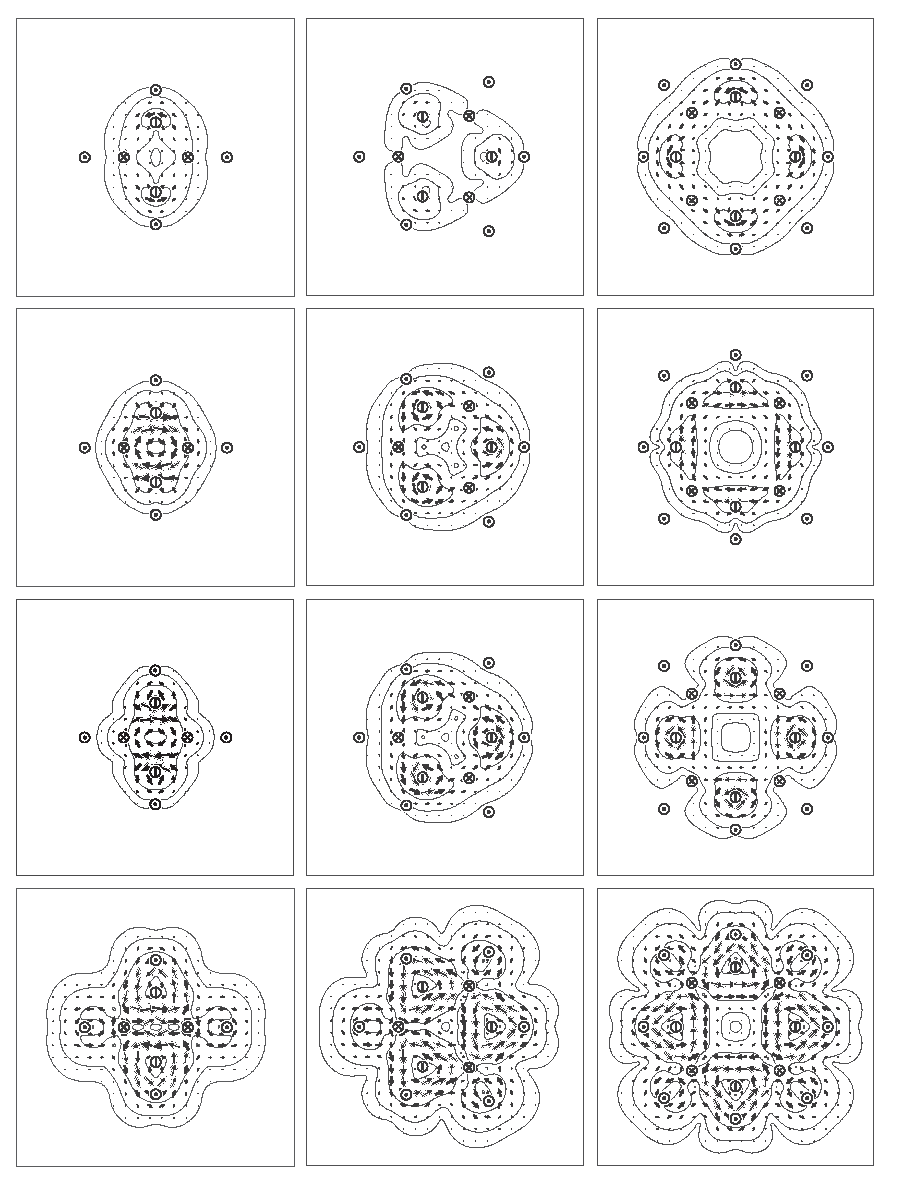
\includegraphics{huckel/figures/fig4.eps}
\end{center}
\caption{Current density induced by a perpendicular external magnetic field in the molecules B$_2$N$_2$H$_4$ (\textbf{1}, planar), B$_3$N$_3$H$_6$ (\textbf{2}), B$_4$N$_4$H$_8$ (\textbf{3}) (left to
right), partitioned as contributions from (top to bottom) the \mbox{HOMO-1}, HOMO, $\pi$ and $\sigma$ orbitals, calculated by the RHF/6-31G** ipsocentric approach. Where the \mbox{HOMO-1} and HOMO are degenerate, the map shows the summed contribution of the pair. Contributions are plotted at one bohr above the molecular plane. Anti-clockwise circulations are
diatropic, clockwise circulations paratropic. Nitrogen, boron and hydrogen centers are denoted by circles containing a bar, cross or dot, respectively.}
\label{ch5.fig.f04}
\end{figure}
For each molecule, the maps show HOMO, \mbox{HOMO-1} and the total $\pi$ and $\sigma$ contributions to the induced current density plotted in a plane one bohr above
that of the nuclei. As Figure \ref{ch5.fig.f04} shows, all three systems, in contrast to the carbocycles, have multi-center patterns of local diatropic $\pi$ circulations centered on the
nitrogen atoms. In B$_3$N$_3$H$_6$, the nitrogen-centered $\pi$ circulations arise entirely from the four electrons of the doubly degenerate HOMO:
the total $\pi$ and HOMO maps are visually indistinguishable, and the contribution of the \mbox{HOMO-1} is negligible. In B$_2$N$_2$H$_4$ and B$_4$N$_4$H$_8$, the
nitrogen-centered $\pi$ circulations arise from a combination of the inner paratropic HOMO and the outer diatropic \mbox{HOMO-1} currents. As the localized
$\sigma$ and $\pi$ currents rotate in the same sense, they are reinforced in all three molecules. Maps of total current density (not shown) plotted for the puckered optimum
geometry of B$_2$N$_2$H$_4$ at a height of 1 $a_0$ above the nitrogen atoms and parallel to the median nuclear plane show the same general features:
the localized nature of the current density is not critically dependent on planarity.

\subsection{Localized Orbital Analysis}
Further analysis using Pipek-Mezey localization of the canonical molecular orbitals \cite{r31} demonstrates the strong generic similarity of all three systems.
The localized orbitals of B$_{N/2}$N$_{N/2}$H$_N$ are $N$ core $1s$ orbitals on the heavy atoms, $N/2$ BN localized $\sigma$ bonding orbitals,
$N/2$ NH and $N/2$ BH localized $\sigma$ bonding orbitals and $N/2$ $\pi$ orbitals that are essentially nitrogen-localized $\pi$ lone
pairs. In this analysis nitrogen-centered $\pi$ currents arise naturally as circulations in the lone pairs. The $\sigma$ currents shown
in Figure \ref{ch5.fig.f04} for B$_2$N$_2$H$_4$, B$_3$N$_3$H$_6$ and B$_4$N$_4$H$_8$ have nodes at the boron sites. In the localized-orbital picture, the prominent
``triangular'' diatropic circulations around the nitrogen atoms arise from the three bonds meeting at nitrogen, each
deltoid constituting a six-electron diatropic circulation. In the carbocycles, the $\sigma$ currents are more uniformly distributed
over all the heavy atoms, but are still spatially localized \cite{r32}. The main difference in the magnetic response between
carbocycles and azabora-heterocycles is that the $\pi$ ring currents of one class are absent in the other. This distinction
is clear from the computed current-density maps, which are fully compatible with the qualitative analysis based
on symmetry and electronegativity. One and the same ipsocentric molecular orbital picture explains both the current in
the carbocycle and the lack of current in the heterocycle.

\subsection{Valence Bond Calculations on Azabora-Heterocycles}
As the localization of density on electronegative nitrogen centers is a key factor in the simple H\"uckel model of ring current
quenching, it is important to verify this qualitative difference between carbocyclic and azabora-heterocyclic systems
by using more sophisticated theoretical methods. Accordingly, \textit{ab initio} Valence Bond Configuration Interaction (VBCI)
calculations, in which many structures are used, and Valence Bond Self Consistent Field (VBSCF) \cite{r33} calculations, in
which both orbitals and structure coefficients are optimized, were performed on planar B$_2$N$_2$H$_4$ (\textbf{1}), B$_3$N$_3$H$_6$ (\textbf{2}) and
B$_4$N$_4$H$_8$ (\textbf{3}) with the 6-31G** basis set. All were carried out by using TURTLE \cite{r34}, as implemented in the GAMESS-UK
package \cite{r35}.

The wave function in the Valence Bond calculations consists of a Hartree-Fock $\sigma$ core in structures with singly occupied
$\pi$ orbitals. From a chemical point of view, these different structures can be seen as different bonding arrangements.
All possible structures that can be generated by using the occupied atomic orbitals were used in the VBCI
wave function, including chemically irrelevant ones. For B$_2$N$_2$H$_4$ there are 20 possible structures which arise from the
20 ways of distributing four electrons over four $p$ orbitals to give a singlet. For B$_3$N$_3$H$_6$ 175 structures are possible, and
for B$_4$N$_4$H$_8$ there are 1764. A VBCI calculation will show which bonding arrangements are preferred.
However, the VBCI wave function, owing to its fixed atomic orbital basis set, does not present a compact description
of the wave function as orbital optimization and correlation effects are intermixed. Therefore the most important
structures in the VBCI calculations were used to construct a VBSCF wave function without imposing restrictions on the
orbitals. From the coefficients in the VBCI wave functions the weights \cite{r36}, and thus the importance of each structure,
may be derived. For \textbf{1}-\textbf{3}, the most important structure types are shown in Figure \ref{ch5.fig.f05} with their respective weights.
\begin{figure}
\begin{center}
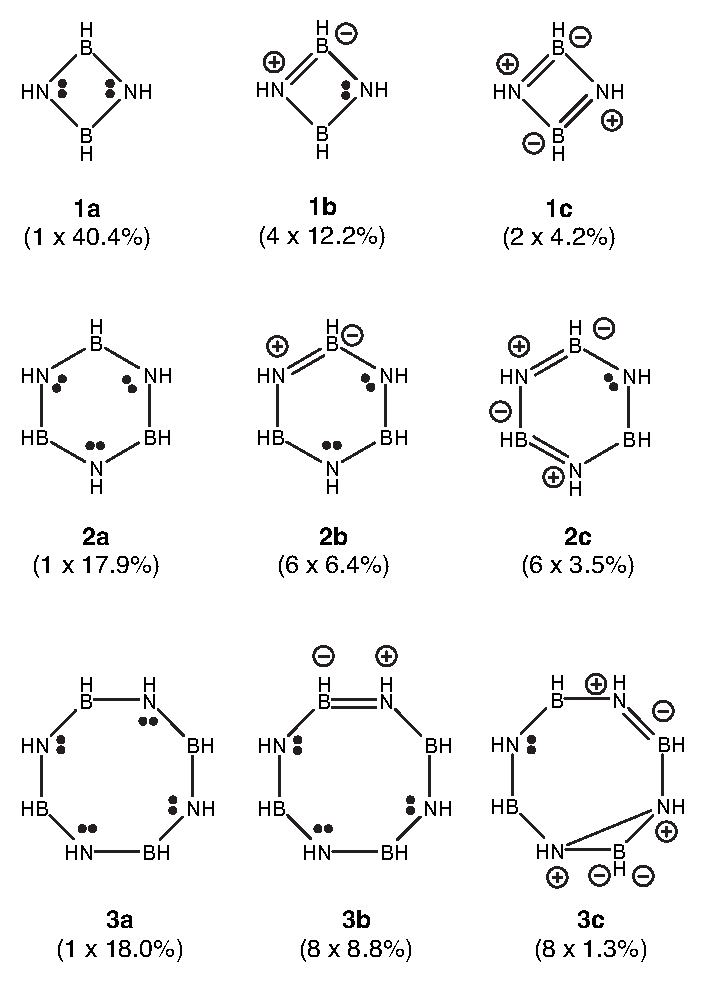
\includegraphics[scale=0.98]{huckel/figures/fig5.eps}
\end{center}
\caption{The most significant symmetry-distinct VBCI structures of
B$_2$N$_2$H$_4$ (\textbf{1}), B$_3$N$_3$H$_6$ (\textbf{2}) and B$_4$N$_4$H$_8$ (\textbf{3}) with the total weight of the combined
set in parentheses.}
\label{ch5.fig.f05}
\end{figure}
From these weights it appears that several structures contribute to the total wave function.

Subsequently, for B$_2$N$_2$H$_4$, the sets of structures of each kind were separately optimized in VBSCF calculations without imposing any
restrictions on the orbitals. The resulting energies of the first (\textbf{1a}:  160.722209 $E_\mathrm{h}$) and the second
(\textbf{1b}:  160.721245 $E_\mathrm{h}$) were very similar, with the first structure, having two different orbitals on each nitrogen atom
(see Figure \ref{ch5.fig.f06}), slightly more favorable.

\begin{figure}
\begin{center}
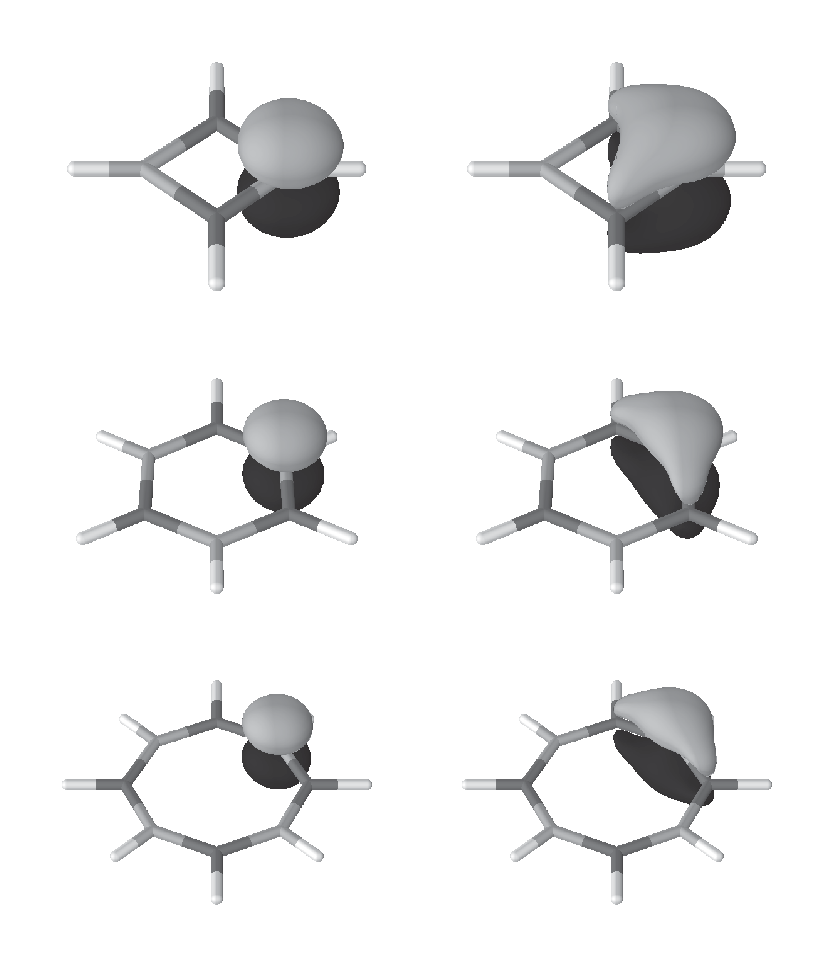
\includegraphics{huckel/figures/fig6.eps}
\end{center}
\caption{The singly occupied $p$ orbitals of B$_2$N$_2$H$_4$ (\textbf{1}), B$_3$N$_3$H$_6$ (\textbf{2}) and B$_4$N$_4$H$_8$ (\textbf{3}), respectively,
which correspond to the structures \textbf{1a}, \textbf{2a} and \textbf{3a} (see Figure \ref{ch5.fig.f05}). Orbitals from the left and right of the picture together
form the correlated lone pair on the nitrogen atom.}
\label{ch5.fig.f06}
\end{figure}

A VBCI calculation was then performed on the first two sets of structures (\textbf{1a}+\textbf{1b}), each with their own optimized
orbitals. This calculation gave the same energy as the single structure VBSCF calculation (\textbf{1a}), whereas the overlap between
set one (\textbf{1a}) and set two (\textbf{1b}) was over 99.9\%. This means that the VBSCF calculations converge to the same
wave function, which is most aptly described as nitrogen atoms, each with a correlated pair of $\pi$ electrons. The conclusion
is that there is no resonance energy and thus no resonance \cite{r37}. Similar results were obtained for B$_3$N$_3$H$_6$ (\textbf{2}) \cite{r37}
and B$_4$N$_4$H$_8$ (\textbf{3}).

These calculations show the same tendency as both the H\"uckel and the ring current calculations, that is, localization
of electrons on the nitrogen atoms. In fact, the Valence Bond results show that the ground states of B$_2$N$_2$H$_4$ (\textbf{1}), B$_3$N$_3$H$_6$
(\textbf{2}) and B$_4$N$_4$H$_8$ (\textbf{3}) correspond to the structures \textbf{1a}, \textbf{2a} \cite{r37} and \textbf{3a}, respectively.

\section{Conclusions}

Given the success of the simple one-parameter model in pointing out qualitative differences in current patterns between
carbo- and azabora-cycles, it is natural to ask about its predictions for other systems, for example, X$_{N/2}$Y$_{N/2}$H$_N$-
where does the borderline between ``aromatic'' and ``non-aromatic'' occur in this picture? The crudest form of the
model shows a change from global circulation to localized currents by a strong reduction in the magnitude of ring current
from $\eta$=0 to $\eta$=1; this variation is sigmoidal (Figure \ref{ch5.fig.f07})
\begin{figure}
\begin{center}
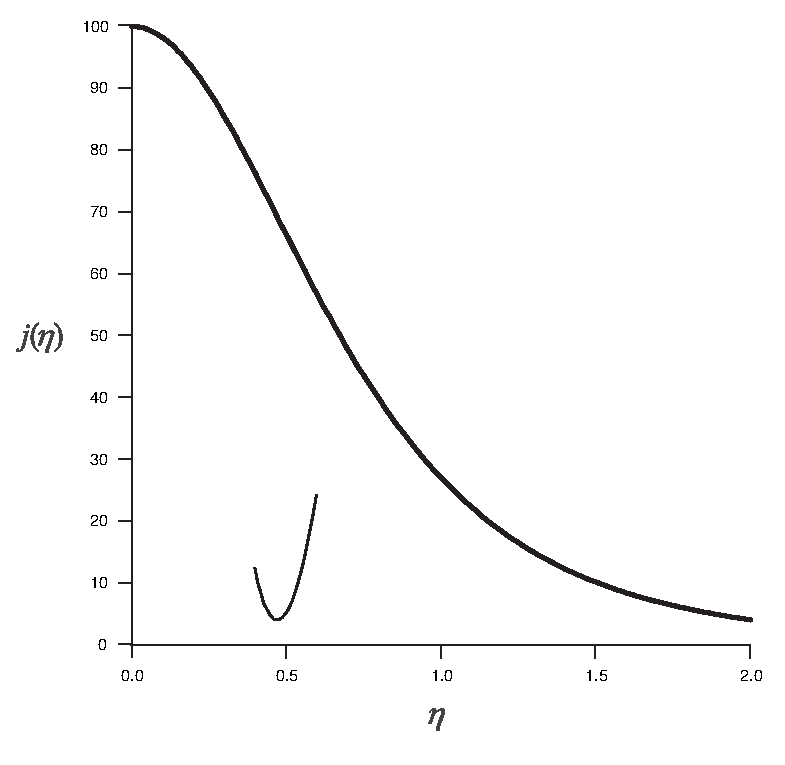
\includegraphics{huckel/figures/fig7.eps}
\end{center}
\caption{
Variation of ring current, $j$, with electronegativity parameter, $\eta$,
in the H\"uckel-London treatment of the X$_3$Y$_3$ cycle. $j(\eta)$ is the ring current
for a regular hexagonal cycle with alternating coulomb parameters
$\alpha \pm \eta \beta$ as a percentage of the current for the same cycle with $\eta$=0. The
inset curve (not to scale) shows the variation of the first derivative d$j(\eta)$/d$\eta$ near $\eta$=0.5.
}
\label{ch5.fig.f07}
\end{figure}
with a point of inflection, where current will be most sensitive to variation in $\eta$, at $\eta \approx$ 0.5, where $\eta$ represents the deviation
from the average electronegativity, that is, $| \alpha_\mathrm{X}- \alpha_\mathrm{Y} | 2\beta$. A rule of thumb is that $\alpha_\mathrm{X}$
varies with the difference in electronegativity between X and C: $(\alpha_\mathrm{X} - \alpha_\mathrm{C})/\beta \approx \chi_\mathrm{X}-\chi_\mathrm{C}$
for X as a one-electron donor and  $(\alpha_\mathrm{X} - \alpha_\mathrm{C})/\beta \approx 1 + \chi_\mathrm{X}-\chi_\mathrm{C}$ as a two-electron
donor \cite{r22a}. Inflection at $\eta\approx$ 0.5 is consistent with indications for X$_3$Y$_3$ 6$\pi$ systems from ring current maps \cite{r02} and
NICS calculations \cite{r27c}: systems in which the electronegativity/coulomb-parameter difference between X and Y is 1 or
more on the Pauling scale lack ring currents (B$_3$O$_3$H$_3$ \cite{r02,r27c}, B$_3$N$_3$H$_6$ \cite{r02,r27c}, Al$_3$N$_3$H$_6$ \cite{r27c} and
Al$_3$P$_3$H$_6$ \cite{r27c}), whereas those with differences of half a unit or less may (C$_3$N$_3$H$_3$ \cite{r02,r27c} and B$_3$P$_3$H$_6$ \cite{r27c})
or may not (B$_3$S$_3$H$_3$ \cite{r27c}) show global currents. This uniform trend lends support to the expectation that orbital-based models should be able to
account for the subtleties of ring current in the range of aromatic, non-aromatic and anti-aromatic heterocycles, and is a strong argument for
using methods in which the orbital contributions themselves have a clear physical basis.

\section*{Addendum}
The results and discussion presented in this chapter have been used by other researchers, both for experimental work \cite{ae01,ae02,ae03} as well as for computational analysis \cite{ac01,ac02,ac03,ac04,ac05}. The most recent is an article of Wang \textit{et al.} \cite{ae01}, in which they describe the concept of replacing the CC unit with its isoelectronic BN unit in organic $\pi$-systems. 

In this chapter, a simple H\"uckel model is used to analyze the difference in character of the $\pi$ electron system of CC compared to BN bonds. The same type of model has been used by van den Heuvel and Soncini \cite{ac02}. They apply the model to graphene and subsituted derivatives, referred to as bond-decoration by the authors. Graphene contains a single layer of carbon atoms structured in a honeycomb (hexagonal) lattice.

\section*{Acknowledgements}
L.W.J. acknowledges financial support from the Royal Society of Chemistry's Journals Grants for International Authors Programme (0301433).
R.W.A.H. acknowledges financial support from the Netherlands Organization for Scientific Research (NWO), grant 700.53.401. P.W.F, A.R. and
A.S. thank the EU for financial support from the Framework V programme (RTN Contract HPRN-CT-2002-00136 ``WONDERFULL'').
C.D. thanks the Royal Society for a University Research Fellowship and P.W.F. for a Royal Society/Wolfson Research Merit Award.

\bibliography{huckel}
\bibliographystyle{../main/achemso}
